\documentclass[a4paper, 12pt]{article}
\usepackage{graphicx}
\usepackage{fancyhdr}
\usepackage[a4paper, top=3cm, left=3cm, right=2cm, bottom=2cm]{geometry}
\usepackage{xcolor} % Paket untuk warna
\usepackage{setspace} % Paket untuk spasi
\usepackage{xcolor, color}
\usepackage{setspace}
\usepackage{titlesec,titletoc}

\linespread{1.25} % Mengatur spasi seluruh dokumen

% Custom commands
\definecolor{sectionColor}{rgb}{0.87, 0.92, 0.96}

% Helper command for full-width section background
\newcommand{\sectionformat}[1]{%
    \noindent\colorbox{sectionColor}{\parbox{\dimexpr\textwidth-2\fboxsep}{\thesection\quad#1}}%
}

%custom style for section title
\titleformat{\section}
    {\normalfont\Large\bfseries}
    {}
    {0em}
    {\sectionformat}

\begin{document}

% Title
\begin{center}
    \textcolor[rgb]{0.176, 0.455, 0.710}{%
        \huge \textbf{%
            Analisis Koefisien Restitusi pada Bola Berbasis ESP8266 Dengan Protokol MQTT Melalui Antarmuka Grafis Secara Realtime
        }%
    }
\end{center}

\section{Tujuan}
\begin{enumerate}
    \item Merancang dan membangun sistem pengukur koefisien restitusi berbasis ESP8266 dengan protokol MQTT
    \item Mengetahui pengaruh elastisitas bola terhadap jumlah pantulan yang terukur oleh sensor HCSR04
    \item Mengetahui nilai koefisien restitusi dari setiap pantulan bola yang dihasilkan
\end{enumerate}

\section{Dasar Teori}
\subsection{Koefisien Restitusi}
\subsection{Elastisitas Bola}
\subsection{Mikrokontroler ESP8266}
\subsection{Sensor HCSR04}
\subsection{Protokol MQTT}

\section{Metode Percobaan}

\subsection{Alat dan Bahan}
\begin{table}[!ht]
    \centering
    \caption{Alat yang digunakan}
    \label{tab:alat}
    \begin{tabular}{|l|l|l|}
        \hline
        \textbf{No} & \textbf{Alat Penelitian} & \textbf{Jumlah Alat} \\
        \hline
        1 & Laptop & 1 buah \\
        \hline
        2 & ESP8266 & 1 buah \\
        \hline
        3 & HCSR-04 & 1 buah \\
        \hline
        4 & Kabel Jumper & Secukupnya \\
        \hline
        5 & Akrilik & Secukupnya \\
        \hline
        6 & Pipa Besi & Secukupnya \\
        \hline
        7 & Mur dan Baut & Secukupnya \\
        \hline
        8 & Penyambung Pipa & Secukupnya \\
        \hline
        9 & \textit{Software} Arduino & - \\
        \hline
    \end{tabular}
\end{table}

\begin{table}[!ht]
    \centering
    \caption{Bahan yang digunakan}
    \label{tab:bahan}
    \begin{tabular}{|l|l|l|}
        \hline
        \textbf{No} & \textbf{Bahan Penelitian} & \textbf{Jumlah Bahan} \\
        \hline
        1 & Bola Tenis Meja & 1 buah \\
        \hline
        2 & Bola Bekel & 1 buah \\
        \hline
        3 & Bola Sepak Karet & 1 buah \\
        \hline
        4 & Bola Plastik & 1 buah \\
        \hline
        5 & Bola Tenis lapang & 1 buah \\
        \hline
    \end{tabular}
\end{table}

\subsection{Prosedur Percobaan}

\begin{figure}[!ht]
    \centering
    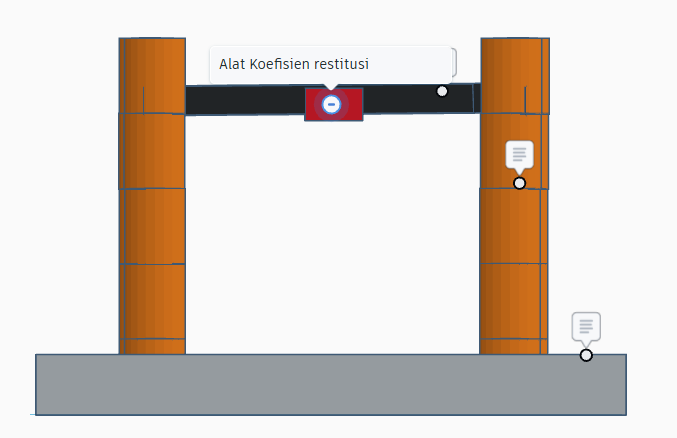
\includegraphics[width=0.5\linewidth]{Desain Alat.png}
    \caption{Desain Alat}
    \label{fig:desain-alat}
\end{figure}

\begin{figure}[!ht]
    \centering
    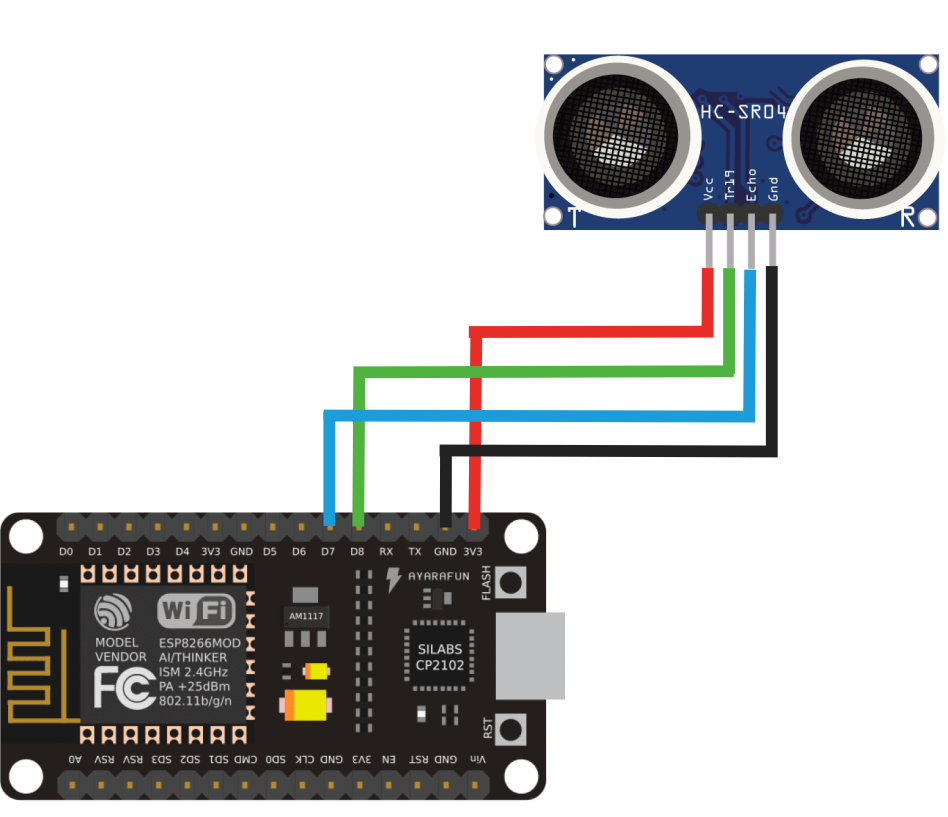
\includegraphics[width=0.5\linewidth]{Rangkaian Elektronika.png}
    \caption{Rangkaian Elektronika}
    \label{fig:rangkaian-elektronika}
\end{figure}

\section{Data dan Analisis Pengujian}

\section{Referensi}

\end{document}
